% Rutsky_FSF_and_OSS_movements_Outline.tex
% Help Sheet on Free Software and Open Source movements for English seminars.
% Vladimir Rutsky <altsysrq@gmail.com>
% 25.03.2009

\documentclass[10pt,a4paper]{article}

% Spaces after commas.
\frenchspacing
% Minimal carrying number of characters,
\righthyphenmin=2

% Encoding support.
\usepackage[utf8x]{inputenc}
\usepackage{url}
\usepackage[russian,english]{babel}

% For embedded images.
%\usepackage{color}
\usepackage[pdftex]{graphicx}

% From K.V.Voroncov Latex in samples, 2005.
\textheight=24cm   % Text height.
\textwidth=16cm    % Text width
\oddsidemargin=0pt % Left side indention.
\topmargin=-1.5cm  % Top side indention.
\parindent=24pt    % Paragraph indent.
\parskip=0pt       % Distance between paragraphs.
\tolerance=2000
%\flushbottom       % Page height aligning.


% Numerating sections with Roman numerals.
\renewcommand \thesection{\Roman{section}}

% Smaller interval.
%\renewcommand{\baselinestretch}{0.7}
% TODO
%\newcommand{\bee}{\begin{enumerate}\setlength{\itemsep}{-0.7mm}}
\newcommand{\bee}{\begin{enumerate}}
\newcommand{\ene}{\end{enumerate}}
%\newcommand{\bit}{\begin{itemize}\setlength{\itemsep}{-0.7mm}}
\newcommand{\bit}{\begin{itemize}}
\newcommand{\eit}{\end{itemize}}

\title{Free Software and Open Source movements \\ Outline}
\author{Rutsky\,V., 3057/2}
%\date{}

\begin{document}

% Title.
\maketitle

% Content.

\section{Introduction}
\bee
  \item Intellectual property (IP): copyrights, trademarks, patents, licenses
  \bee
    \item Intellectual property rights (IPR)~--- right of owning of non-rival goods (creations of the mind).
    \item IPR gives temporary monopoly rights. After time is out created work became public domain.
    \item Objective of IPR: growth of technologies by stimulating process of giving to the World intellectual creations.
    \item Different types of intellectual property: 
    \bit
      \item copyrights~--- exclusive rights to publication, distribution and adaptation of work.
      ``Moral right''.
      Applies to any expressible form of an idea or information that is substantive and discrete 
      (such as poems, movies, dances, paintings, software, radio\ldots)
      Berne Convention (1886): every written text is automatically copyrighted.
      Buenos Aires Convention (1910): every written text with note is copyrighted (US).
      \item trademarks~--- signs for identification of product/service unique origin.
      Requiered to exclusevely identify the commercial source or origin of product/service, it's a badge of origin.
      \item patents~--- exclusive rights granted to an inventor for a limited period of time in exchange 
      for a disclosure of an invention.
      If inventors did not have the legal protection of patents, they would prefer to keep their inventions secret.
    \eit
    \item Criticims: 
    \bit
      \item ideas are not unique, and few people at the same time can invent something similar,
      \item hard to divide what inventions are obvious and what is not.
    \eit
    \item IPR and software: good idea, bad implementation. 
    Using unpatented ideas frightening because of possibility that someone will patent them later.
    Strange patents such as mouse double click. 
    Patent trolls.
    Software world is too flexible and mobile.
  \ene
  \item Software categories
  \bee
    \item Diagram showing relations between software categories.
    % TODO
    
    \DeclareGraphicsRule{.pdftex}{pdf}{.pdftex}{}
    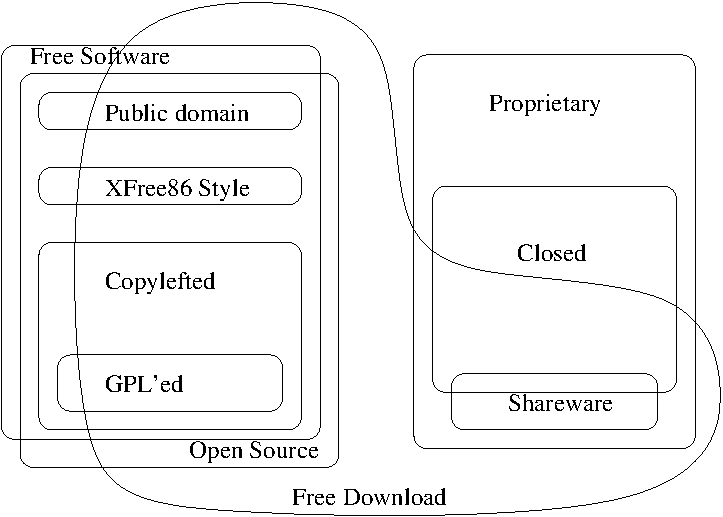
\includegraphics{images/category.pdf}
    \item ``Commercial software'' is not equal to ``proprietary software''.
  \ene
\ene

\section{Free Software movement}
\bee
  \item How the movement was started
  \bee
    \item Richard Matthew Stallman. Born in 1953, graduated with BA in Physics at Harvard University in 1974, 
    at the time of studying Harvard he worked in MIT AI Labs.
    \item After U.S. Copyright Act of 1976 number of proprietary programs in 1970~--1980 grew, 
    to prevent of being used on competitors' computers.
    \item In 1980, Stallman and some other hackers at the AI Lab were refused access to the source code for the software 
    of the first laser printer, that Xerox company has gifted to them. 
    Stallman had modified the software on an older printer for more comfortable use and wasn't able to do so on Xerox printer.
    This experience convinced Stallman of people's need to be free to modify the software they use.
  \ene
  \bee
    \item Idea of Free Software and Free Software Definition, four freedoms of Free Software:
    \bee
      \item[Freedom 0:] The freedom to run the program, for any purpose.
      \item[Freedom 1:] The freedom to study how the program works, and adapt it to your needs.
      \item[Freedom 2:] The freedom to redistribute copies so you can help your neighbor.
      \item[Freedom 3:] The freedom to improve the program, and release your improvements 
      (and modified versions in general) to the public, so that the whole community benefits.
    \ene
    \item Social aspect of Free Software and the goal: it is a philosophy to make World better.
    Social solidarity: sharing and cooperation.
  \ene
  \item GNU Project (1983). Free software, mass collaboration project to develop replacement for non-free software.
  \item GNU OS (1984)
  \bee
    \item GNU. GNU's Not Unix. Compatible alternative to proprietary Unix.
    \item Linus Torvalds, born in 1969.
    \item Linux project and GNU/Linux OS. Filling gap of GNU OS.
  \ene
  \item Free Software Foundation (1985). Non-profit corporation to support free software movement.
  \item Free software protectors~--- licenses
  \bee
    \item Copyleft. 
    It is a copyright with addition that work can be modified and redistributed with modifications 
    but only with the same restrictions.
    \item GNU General Public License. Strong copyleft license.
  \ene
\ene

\section{Open Source movement}
\bee
  \item Open source is an approach to design, development, and distribution offering practical accessibility 
  to a product's source. It is a ``practical part'' of Free Software.
  \item Open source was born in the process of evolution of software development techniques.
  \item Eric Steven Raymond, born in 1957. 
  He had a lot of programming practice and wrote ``The Cathedral and the Bazaar'' (1997): 
  analysis of software development by closed group vs. massive and partially decentralized development, 
  development of Emacs vs development Linux.
  ``Given enough eyeballs, all bugs are shallow.''~--- ``Linus' Law''.
  \item 1998. Netscape Communications Corporation releases their popular Netscape Communicator Internet suite as free software.
  \item 1998. Focusing on source code without much attention to free software goals: Bruce Perens and Eric Raymond founded 
  Open Source Initiative.
  \item Open Source Definition:
  \bee
    % TODO: do normal counter.
    \item[1.] Free redistribution.
    \item[2.] Source code.
    \item[3.] Derived works.
    \item[4.] Integrity of the author's source code. 
    (Distributing modifications as patches.)
    \item[5.] No discrimination against persons or groups.
    \item[6.] No discrimination against fields of endeavor.
    (Must not be restricted to be used in business for example.)
    \item[7.] Distribution of license.
    (No additional license restrictions.)
    \item[8.] License must not be specific to a product.
    (No restrictions to use software in particular software distribution.)
    \item[9.] License must not restrict other software.
    (No restrictions like all software that come with this program must be open source.)
    \item[10.] License must be technology-neutral.
  \ene
  \item Open Source is a powerful and reliable software.
  \item Advantages:
  \bit
    \item Open source software is a well written software and provide high quolity of services, 
    otherwise someone else will be able to provide better open source solution from their code or better services.
    Open source software must be best software to be successful.
    \item No monopolies, all ideas and technologies correctness and quality can be controlled by community.
    \item Better bug fixing scheme than in proprietary model.
    \item Very flexible solutions, no limitations in changing software for needs of end user.
    Software will not ``die'' when get unsupported by original developers.
    \item Cheap development for good projects due to community support.
    \item No spyware and malware.
  \eit
  \item Free Software and Open Source are different.
  Free Software fights for personal freedoms to make World better, 
  Open Source is an effective development approach.
\ene

\section{Licenses}
\bee
  \item Copyleft vs. permissive licenses vs. public domain. Common rights that they give.
  \item GPL-like: GNU Lesser GPL, GNU Affero GPL, GNU Free Documentation License.
  \item BSD-like: BSD, MIT, Boost Software License, Apache License.
  \item CreativeCommons. BY/BY-SA/BY-ND/BY-NC/BY-NC-SA/BY-NC-ND.
\ene

\section{Free Software, Open Source and profit}
\bee
  \item ``Free'' is not about price! R.~Stallman made some money on selling GNU Emacs.
  \item Selling program binary is mostly unprofitable if you are not Big Monopolist Corporation.
  \item Open Source business models:
  \bee
    \item Redistribution and support. 
    MySQL.
    \item Double licensing. 
    Trolltech~Qt, Berkeley~DB.
    \item Free Open Source editions and commercial enterprize editions.
    Red~Hat (Fedora and Red~Hat Enterprise Linux), Novell (openSUSE and SUSE Linux), Sun (OpenSolaris and Solaris)
    \item Implementing programs/servers solutions. Zend Corporation.
    \item Partnerships with other companies. Mozilla and Google.
  \ene
\ene

\section{Success stories}
\bee
  \item End user examples: operating systems, servers, supercomputers, desktop, web, 
  science tools, a lot of developer tools\dots
  Well working Free and Open Source software are everywhere.
  \item Corporation examples: Cygnus Solutions, Canonical~Ltd. Red~Hat, Mozilla Corporation, 
  Qt~Software, Sun~Microsystems, Google\dots
  Biggest corporations gaining profit using and developing Free and Open Source software.
\ene

\section{Conclusion}
\bee
  \item Free Software is a way to make world better and may require some sacrifices.
  \item Open Source is a quality guarantee and a proved model of software development.
  \item It is possible to gain money and work for freedom.
\ene

\section*{Sources}
  \bit
    \item \url{http://www.fsf.org/}~--- Free Software Foundation
    \item \url{http://www.opensource.org/}~--- Open Source Initiative
    \item \url{http://en.wikipedia.org/wiki/Portal:Free_software}~--- Wikipedia Free Software Portal
  \eit

\end{document}
